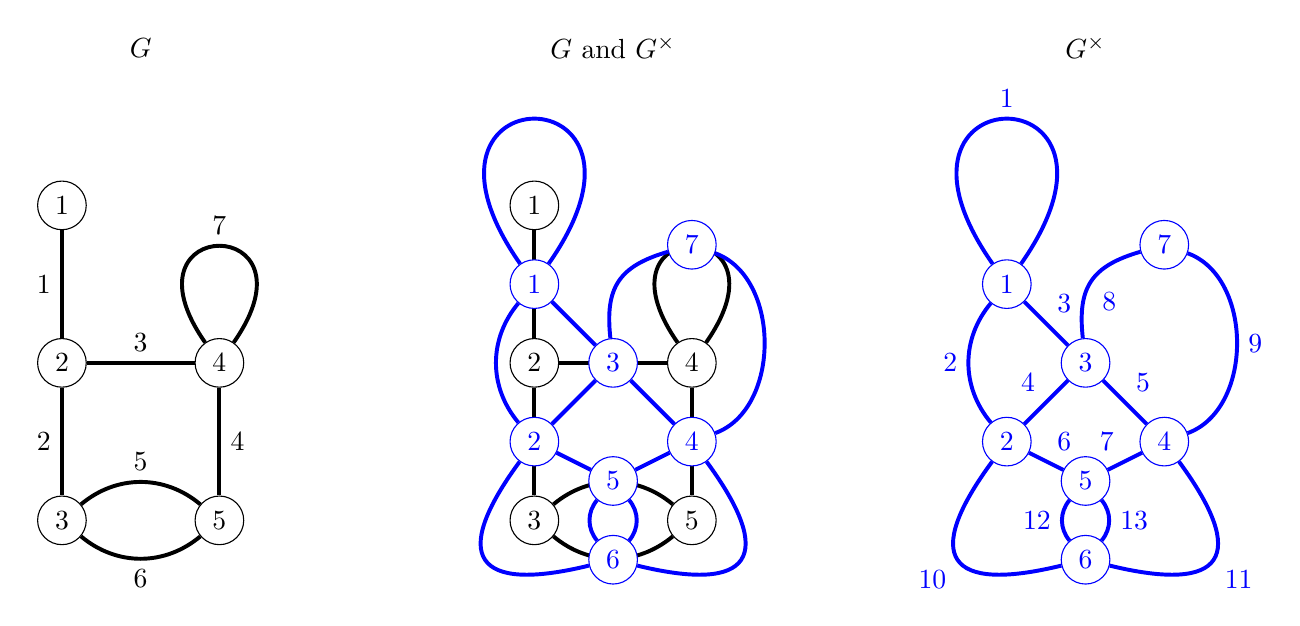
\begin{tikzpicture}
	\begin{scope}[xshift=0cm, yshift=0cm]
		\node (G) at (1, 6) {$G$};

		\node[circle, draw] (a1) at (0, 4) {1};
		\node[circle, draw] (a2) at (0, 2) {2};
		\node[circle, draw] (a3) at (0, 0) {3};
		\node[circle, draw] (a4) at (2, 2) {4};
		\node[circle, draw] (a5) at (2, 0) {5};
	
		% Draw the edges between nodes with labels
		\draw[line width=0.5mm] (a1) -- node[left] {1} (a2);
		\draw[line width=0.5mm] (a2) -- node[left] {2} (a3);
		\draw[line width=0.5mm] (a2) -- node[above] {3} (a4);
		\draw[line width=0.5mm] (a4) -- node[right] {4} (a5);
		\draw[line width=0.5mm] (a3) to[bend left=40] node[above] {5} (a5);
		\draw[line width=0.5mm] (a3) to[bend right=40] node[below] {6} (a5);
		\draw[line width=0.5mm] (a4) to[in=125,out=55,loop, min distance=2cm] node[above] {7} (a4);
	\end{scope}

	\begin{scope}[xshift=6cm, yshift=0cm]
		\node (G) at (1, 6) {$G$ and $G^\times$};

		\node[circle, draw] (a1) at (0, 4) {1};
		\node[circle, draw] (a2) at (0, 2) {2};
		\node[circle, draw] (a3) at (0, 0) {3};
		\node[circle, draw] (a4) at (2, 2) {4};
		\node[circle, draw] (a5) at (2, 0) {5};
	
		% Draw the edges between nodes with labels
		\draw[line width=0.5mm] (a1) -- (a2);
		\draw[line width=0.5mm] (a2) -- (a3);
		\draw[line width=0.5mm] (a2) -- (a4);
		\draw[line width=0.5mm] (a4) -- (a5);
		\draw[line width=0.5mm] (a3) to[bend left=40] (a5);
		\draw[line width=0.5mm] (a3) to[bend right=40] (a5);
		\draw[line width=0.5mm] (a4) to[in=125,out=55,loop, min distance=2cm] (a4);

		\node[circle, draw, color=blue, fill=white] (b1) at (0, 3) {1};
		\node[circle, draw, color=blue, fill=white] (b2) at (0, 1) {2};
		\node[circle, draw, color=blue, fill=white] (b3) at (1, 2) {3};
		\node[circle, draw, color=blue, fill=white] (b4) at (2, 1) {4};
		\node[circle, draw, color=blue, fill=white] (b5) at (1, 0.5) {5};
		\node[circle, draw, color=blue, fill=white] (b6) at (1, -0.5) {6};
		\node[circle, draw, color=blue, fill=white] (b7) at (2, 3.5) {7};
	
		% Draw the edges between nodes with labels
		\draw[line width=0.5mm, color=blue] (b1) to[in=125,out=55,loop, min distance=3cm] (b1);
		\draw[line width=0.5mm, color=blue] (b1) to[bend right=40, min distance=0.5cm] (b2);
		\draw[line width=0.5mm, color=blue] (b1) -- (b3);
		\draw[line width=0.5mm, color=blue] (b2) -- (b3);
		\draw[line width=0.5mm, color=blue] (b3) -- (b4);
		\draw[line width=0.5mm, color=blue] (b2) -- (b5);
		\draw[line width=0.5mm, color=blue] (b5) -- (b4);
		\draw[line width=0.5mm, color=blue] (b3) to[bend left=40, min distance=0.65cm] (b7);
		\draw[line width=0.5mm, color=blue] (b4) to[bend right=70, min distance=0.5cm] (b7);
		\draw[line width=0.5mm, color=blue] (b2) to[bend right=70, min distance=1.5cm] (b6);
		\draw[line width=0.5mm, color=blue] (b4) to[bend left=70, min distance=1.5cm] (b6);
		\draw[line width=0.5mm, color=blue] (b5) to[bend right=40] (b6);
		\draw[line width=0.5mm, color=blue] (b5) to[bend left=40] (b6);
	\end{scope}

	\begin{scope}[xshift=12cm, yshift=0cm]
		\node (G) at (1, 6) {$G^\times$};

		\node[circle, draw, color=blue, fill=white] (b1) at (0, 3) {1};
		\node[circle, draw, color=blue, fill=white] (b2) at (0, 1) {2};
		\node[circle, draw, color=blue, fill=white] (b3) at (1, 2) {3};
		\node[circle, draw, color=blue, fill=white] (b4) at (2, 1) {4};
		\node[circle, draw, color=blue, fill=white] (b5) at (1, 0.5) {5};
		\node[circle, draw, color=blue, fill=white] (b6) at (1, -0.5) {6};
		\node[circle, draw, color=blue, fill=white] (b7) at (2, 3.5) {7};
	
		% Draw the edges between nodes with labels
		\draw[line width=0.5mm, color=blue] (b1) to[in=125,out=55,loop, min distance=3cm] node[above] {1} (b1);
		\draw[line width=0.5mm, color=blue] (b1) to[bend right=40, min distance=0.5cm] node[left] {2} (b2);
		\draw[line width=0.5mm, color=blue] (b1) -- node[above right] {3} (b3);
		\draw[line width=0.5mm, color=blue] (b2) -- node[above left] {4} (b3);
		\draw[line width=0.5mm, color=blue] (b3) -- node[above right] {5} (b4);
		\draw[line width=0.5mm, color=blue] (b2) -- node[above right] {6} (b5);
		\draw[line width=0.5mm, color=blue] (b5) -- node[above left] {7} (b4);
		\draw[line width=0.5mm, color=blue] (b3) to[bend left=40, min distance=0.65cm] node[below right] {8} (b7);
		\draw[line width=0.5mm, color=blue] (b4) to[bend right=70, min distance=0.5cm] node[right] {9} (b7);
		\draw[line width=0.5mm, color=blue] (b2) to[bend right=70, min distance=1.5cm] node[below left] {10} (b6);
		\draw[line width=0.5mm, color=blue] (b4) to[bend left=70, min distance=1.5cm] node[below right] {11} (b6);
		\draw[line width=0.5mm, color=blue] (b5) to[bend right=40] node[left] {12} (b6);
		\draw[line width=0.5mm, color=blue] (b5) to[bend left=40] node[right] {13} (b6);
	\end{scope}
\end{tikzpicture}
